\begin{explanationbox}
\begin{minipage}{\linewidth}
\begin{center}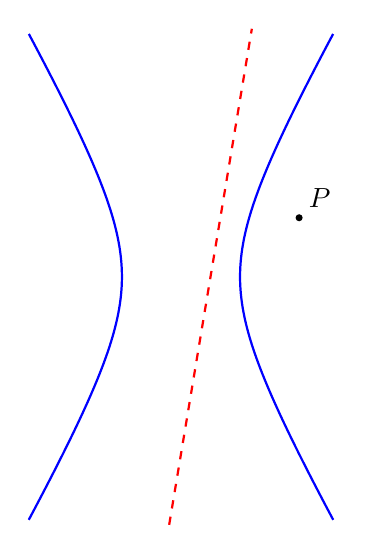
\begin{tikzpicture}[scale=0.75,>=stealth]
\draw[blue,thick,domain=-1.6:1.6,samples=90] plot ({cosh(\x)},{sqrt(3)*sinh(\x)});\draw[blue,thick,domain=-1.6:1.6,samples=90] plot ({-cosh(\x)},{sqrt(3)*sinh(\x)});\draw[red,dashed,thick] (-.2,-4.2)--(1.2,4.2);\fill (2,1) circle (1.7pt) node[above right] {$P$};
\end{tikzpicture}
\end{center}
$x^2-y^2/3=1$ 与点 $P=(2,1)$：红色极线为 $6x-y=3$，但它与双曲线没有实交点，所以原例题的实切点弦不存在。
\end{minipage}
\par\medskip

	\textbf{\textcolor{CExplanation}{一句话直觉}}
	极线是点关于圆锥曲线的“对应直线”：点在曲线上时极线是切线，确有两不同有限实切点时极线才是切点弦。

	\medskip
	\textbf{\textcolor{CExplanation}{核心拆解}}
	\begin{description}[style=nextline, leftmargin=2.8em, labelsep=0.5em, itemsep=0.45em]
		\item[\textbf{要点一（定义替换）：}]
			极线方程由曲线方程通过替换得到：椭圆 $\dfrac{x^2}{a^2}+\dfrac{y^2}{b^2}=1$ 的极线方程为 $\dfrac{x_0x}{a^2}+\dfrac{y_0y}{b^2}=1$，双曲线和抛物线类似。口诀：平方变乘积，一次变平均。
		\item[\textbf{要点二（对称关系）：}]
			配极原理指出：若点 $Q$ 在点 $P$ 的极线上，则点 $P$ 也在点 $Q$ 的极线上，形成点与直线的对偶关系。
	\end{description}

	\medskip
	\textbf{\textcolor{CExplanation}{几何本质（射影对偶）}}
	极点与极线是射影几何中配极变换的实例，本质上是将点映射为直线，且映射是双向的。在解析几何中，这种对偶性通过代数对称性体现。

	\medskip
	\textbf{\textcolor{CExplanation}{代数意义（线性替换）}}
	极线来自对称极化：二次项作双线性替换，一次项取变量与定点坐标的平均值。它不是外点处的一阶泰勒近似；对二次多项式 $S$，极线左端为 $S(P)+\tfrac12\nabla S(P)\cdot(X-P)$。

	\medskip
	\textbf{\textcolor{CExplanation}{考点价值（快速求弦）}}
	\begin{itemize}[leftmargin=*, itemsep=0.5em, topsep=0.4em]
		\item \textbf{考法一（直接求线）：} 已知点 $P$ 和曲线，直接写出极线方程，作为切线（点在曲线上）或切点弦（点在曲线外），避免联立判别式。
		\item \textbf{考法二（对称转化）：} 利用配极原理，通过已知点在另一点的极线上，反向得到新关系，用于求点坐标或直线方程。
	\end{itemize}

	\medskip
	\textbf{\textcolor{CExplanation}{顿悟点}}
	极线方程不用死背，只要记住“平方变乘积，一次变平均”即可；配极原理本质是等式左右对称交换，结果不变。

	\medskip
	\textbf{\textcolor{CExplanation}{使用场景}}
	\begin{itemize}[leftmargin=*, itemsep=0.5em, topsep=0.4em]
		\item \textbf{场景一（切线情形）：} 点在曲线上，直接写出切线方程。
		\item \textbf{场景二（切点弦）：} 先验证两不同有限实切点存在，再写出切点弦方程。
		\item \textbf{场景三（对称转化）：} 利用配极原理将点与线的关系互相推导，简化计算。
	\end{itemize}

\end{explanationbox}
